\documentclass[
  11pt,
  letterpaper,
   addpoints,
   answers
  ]{exam}

\usepackage{../exercise-preamble}
\usepackage{float}
\begin{document}

\noindent
\begin{minipage}{0.47\textwidth}

\includegraphics[width=\textwidth]{../fcfm_die}
\end{minipage}
\begin{minipage}{0.53\textwidth}
\begin{center} 
\large\textbf{Conversión de la Energía y Sistemas Eléctricos } (EL4111-1) \\
\large\textbf{Examen} \\
\small Prof.~Constanza Ahumada - Rodrigo Moreno.\\
\small Prof.~Aux.~Javiera Pacheco - Erik Sáez\\
\small Ayudantes.~Manuel Aceituno - Pamela Acuña - Alvaro Flores\\
\end{center}
\end{minipage}

\vspace{0.5cm}
\noindent
\vspace{.85cm}

\begin{questions}
    %---------------------------------------------------------------
    \question Un motor de inducción trifásico posee los siguientes datos de placa: \(25 \, [\text{kW}]\), 8 polos, \(450 \, [\text{V}_{\text{ff}}]\), \(50 \, [\text{Hz}]\) y está conectado en configuración estrella, este motor se encuentra conectado a un generador sincrono. Sobre el motorde induccion  se ha realizado una prueba de vacío y de rotor bloqueado, con los cuales se obtuvieron los resultados mostrados en la Tabla 1.
    \begin{table}[h!]
        \centering
        \caption{Resultados de la prueba en vacío y de la prueba de rotor bloqueado.}
        \begin{tabular}{|c|c|c|}
            \hline
            \textbf{Medición} & \textbf{Prueba de vacío} & \textbf{Prueba de rotor bloqueado} \\ \hline
            Tensión entre fases \([V_{\text{ff}}]\) & 450 & 120 \\ \hline
            Corriente de línea \([A]\) & 6 & 18 \\ \hline
            Potencia \([W]\) & 480 & 720 \\ \hline
        \end{tabular}
    \end{table}
    
    Por último, con un óhmetro se determinó que la resistencia en corriente continua entre dos terminales del estator es de \(2 \, [\Omega]\). A partir de lo anterior, se pide:
    
    \begin{enumerate}
        \item Calcular los parámetros del circuito equivalente.
        \item Calcular la velocidad de giro, la corriente de la carga, la corriente de línea, la potencia consumida, las pérdidas, el factor de potencia, el rendimiento de la máquina y el torque ejercido por el eje si el deslizamiento a plena carga es del \(6 \, \%\). Considere que se alcanza el régimen permanente.
        \item Considerando que la reactancia Saturada y no saturada son $X_{s}\approx 6.5$ y $X_{ns}\approx 8.9$  . Determinar la tension interna E y el angulo de carga $\sigma$ cuando el generador opera entregando una potencia reactiva de 3 [MVar] con un factor de potencia de 0.8 inductivo y determine el torque mecanico (\textit{Asuma que el generador opera con un voltaje de 24[kV]})
        \item Bosquejar el diagrama fasorial para el punto de operacion anterior e indicar si el generador se encuentra
        subexcitado o sobreexcitado
    \end{enumerate}

    %---------------------------------------------------------------
    \begin{solution}
        \subsection*{Resolucion 1.1}
        Se busca obtener los parámetros del circuito equivalente, primero se analiza la prueba de vacío. ($w_{s} \approx w_{r} \rightarrow s\approx 0$), con lo que luego se tendra que ($r_{2} \rightarrow \infty$).Por tanto, se tiene el siguiente circuito:
        \begin{center}
            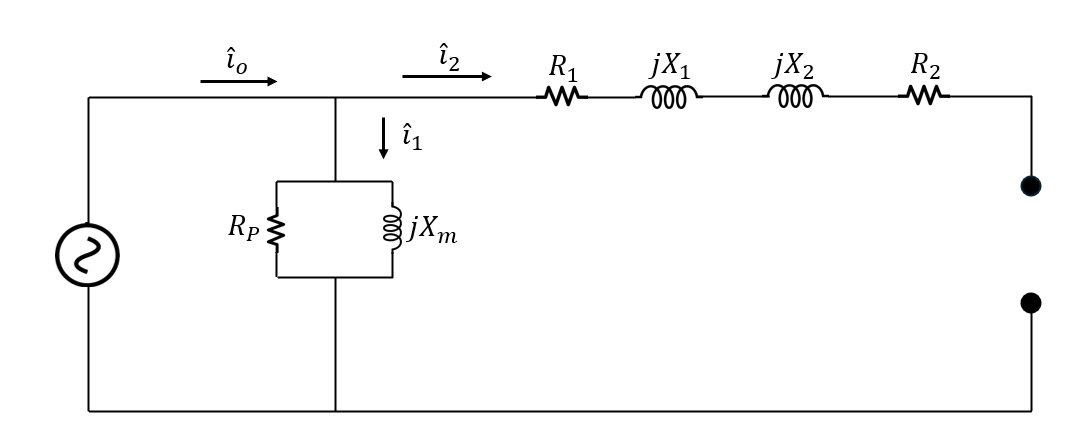
\includegraphics[width=0.6\textwidth]{Auxiliar_9_4}
        \end{center}
        \begin{center}
            \textbf{Figura 1:} Esquema del motor de induccion en su prueba al vacio
        \end{center}
        Para esta situacion se tiene el siguiente set de ecuaciones:
        \begin{align}
            R_{p} &= \frac{V_{fn}^{2}}{P_{0}}\\
            X_{n} &= \frac{V_{fn}^{2}}{Q_{0}}\\
            Q_{0} &= \sqrt{(V_{fn} \cdot I)^{2} - P_{0}^{2}}\\
        \end{align}
        Reemplazando los valores se obtiene que:
        \begin{align}
            R_{p} &= \frac{(450/ \sqrt{3})^{2}[Vfn]}{480[W]} = 140.625[\Omega]\\
            Q_{0} &= \sqrt{\left(\frac{450}{\sqrt{3}} \cdot 6[A]\right)^{2} - 480[W]^{2}} = 1483.10485[VAR]\\
            X_{m} &= \frac{(45 0/\sqrt{3})^{2}[Vfn]}{1483.10485[VAR]} = 45.51263[\Omega]
        \end{align}
        Se obtiene el valor de $r_{1}$ para la prueba de corriente continua:
        \begin{center}
            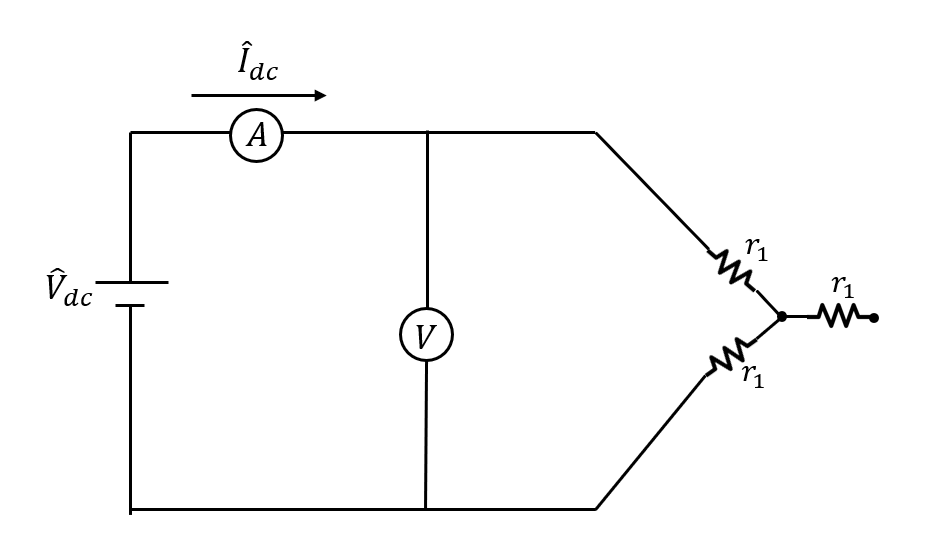
\includegraphics[width=0.5\textwidth]{Auxiliar_9_9}
        \end{center}
        \begin{center}
            \textbf{Figura 2:} Esquema del motor de induccion en su prueba de corriente continua
        \end{center}
        De esta manera se tendra que:
        \begin{align}
            2r_{1} &= \frac{V_{CD}}{I_{DC}}\\
            2r_{1} &= 2[\Omega]\\
            r_{1} &= 1[\Omega]
        \end{align}
        Luego, para la prueba de rotor bloqueado \textit{(Donde $w_r = 0$, por tanto $s = 1$, y por tanto, la resistencia $r_2$ será nula, produciendo un cortocircuito)}, se tendrá el siguiente esquema:        
        \begin{center}
            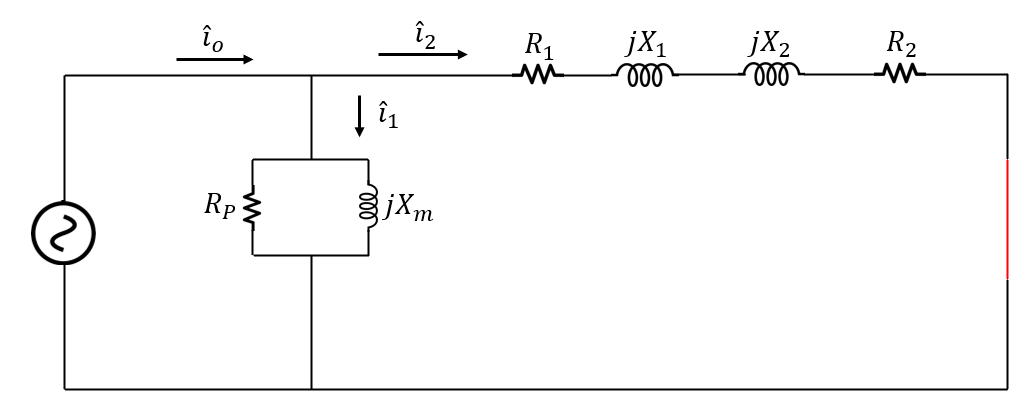
\includegraphics[width=0.6\textwidth]{Auxiliar_9_5}
        \end{center}
        \begin{center}
            \textbf{Figura 2:} Esquema del motor de induccion en su prueba de rotor bloqueado
        \end{center}
        De esta manera se deriva el sigueinte set de ecuaciones:
        \begin{align}
            r_{1} + r_{2} &= \frac{P_{cc}}{i^{2}_{cc}}\\
            X_{1} + X_{2} &= \frac{Q_{cc}}{i^{2}_{cc}}\\
            Q_{cc} &= \sqrt{(V_{cc}i_{cc})^{2} - P_{cc}^{2}}
        \end{align}
        De esta manera, reemplazando sobre los valores que se tienen se concluye que:
        \begin{align}
            r_{1} + r_{2} &= \frac{720[W]}{18[A]^{2}} = 2.22[\Omega]\\
        \end{align}
        Dado que $r_{1} = 1[\Omega]$, luego se tiene que $r_{2} = 1.22[\Omega]$.Por otro lado tenemos que:
        \begin{align}
            Q_{cc} = \sqrt{ \left(\frac{120}{\sqrt{3}} \cdot 18 \right)^{2} - 720^{2}} = 794.41803[VAR]
        \end{align}
        De esta manera se tiene que:
        \begin{align}
            X_{1} + X_{2} &= \frac{794.41803[VAR]}{18[A]^{2}} = 2.4519[\Omega]
        \end{align}
        Con lo que finalmente se obtienen los valores de los parametros del circuito equivalente.
        \subsection*{Resolucion 1.2}
        Se busca el calcular la velocidad de giro, la corriente de la carga, la corriente de línea, la potencia consumida, las pérdidas, el factor de potencia, el rendimiento de la máquina y el torque ejercido por el eje si el deslizamiento a plena carga es del \(6 \, \%\). Considere que se alcanza el régimen permanente.
        \begin{align}
            s = 0.06 
        \end{align}
        Recordemos que s corresponde:
        \begin{align}
            s= \frac{w{s} - w_{r}}{w_{s}} = \frac{n_{s}- n_{r}}{n_{s}}
        \end{align}
        Con lo que considerando que:
        \begin{align}
            n_{s} = \frac{120 \cdot f}{p} = \frac{120 \cdot 50}{8} = 750[rpm]
        \end{align}
        Con lo que podemos obtener el valor de $n_{r}$ como:
        \begin{align}
            s&= \frac{n_{s} - n_{r}}{n_{s}}\\
            0.06 &= \frac{750- n_{r}}{750}\\
            n_{r} &= 705[rpm]
        \end{align}
        Luego se tendra que en [rad/s]:
        \begin{align}
            w_{r} = \frac{2 \cdot \pi \cdot n_{r}}{60} = 73.827[rad/s]
        \end{align}
        La corriente de linea tenemos que recordar el esquema dado por:
        \begin{center}
            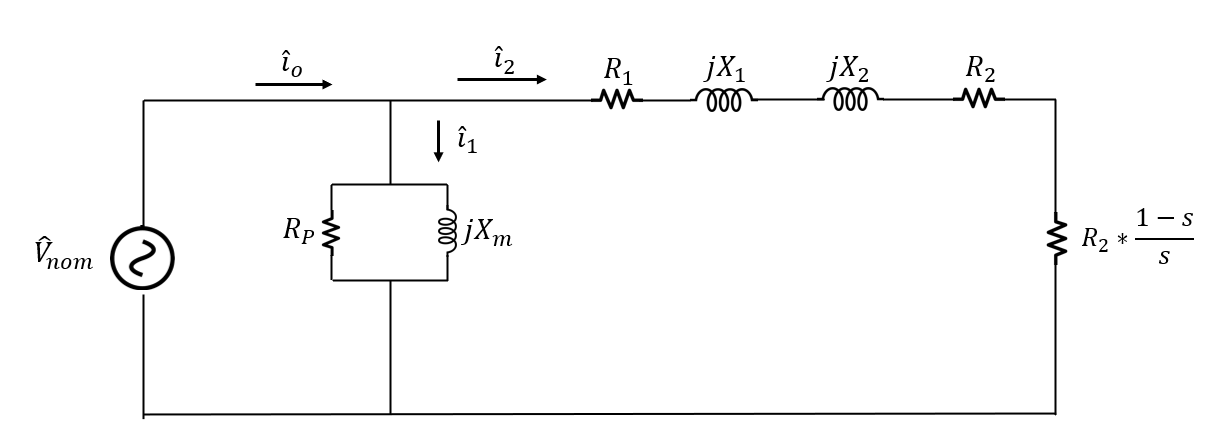
\includegraphics[width=0.6\textwidth]{Auxiliar_9_8}
        \end{center}
        \begin{center}
            \textbf{Figura 5:} Esquema del motor para la corriente de linea $i_{0}$
        \end{center}
        Tenemos que dicha corriente vendra dada por:
        \begin{align}
            \hat{i}_{0} = \frac{\hat{V}_{nom}}{Z_{eq}}
        \end{align}
        Luego tenemos que obtener el valor de la impedancia equivalente, el cual viendo el esquema se tiene:
        \begin{align}
            Z_{eq} = Z_{shunt} // Z_{serie}
        \end{align}
        donde $Z_{shunt}$ es directa de obtener en base a los valores previos, es deicr:
        \begin{align}
            Z_{shunt} &= \left( \frac{1}{R_{p}} + \frac{1}{jX_{m}}\right)^{-1} = 43.3013 \angle 72.0661^{\circ}[\Omega]
        \end{align}
        Luego se debera obtener la impedancia en serie la cual viene dada por:
        \begin{align}
            Z_{serie} = r_{1} + r_{2} + r_{2}\left(\frac{1-s}{s}\right) + j(x_{1} + x_{2}) = 21.1427 \angle 6.65954^{\circ}[\Omega]
        \end{align}
        Por lo que finalmente tendremos que el valor de la impedancia equivalente sera:
        \begin{align}
            Z_{eq} = 43.4013 \angle 72.0661^{\circ} // 21.1427 \angle 6.65954^{\circ} = 16.4855\angle 26.9133^{\circ}[\Omega]
        \end{align}
       La corriente de linea sera:
        \begin{align}
            \hat{i}_{0} = \frac{(450/\sqrt{3} \angle 0^{\circ})}{16.4855 \angle 26.9133^{\circ}} = 15.7598\angle -26.9133^{\circ}[A]
        \end{align}
        Luego se busca obtener la potencia consumida, ademas del factor de potencia, por lo que en base a lo ya obtenido se tiene que:
        \begin{align}
            \hat{S} = \hat{V}_{nom} \cdot \hat{i}_{0}^{*} = 4094.51 \angle 26.9133^{\circ}[VA]
        \end{align}
        Con lo que es posible obtener la potencia activa y reactiva como:
        \begin{align}
            P &= Re(S) = 4094.51\cdot cos(26.9133^{\circ}) = 3651.04[W]\\
            Q &= Im(S) = 4094.51 \cdot sen(26.9133^{\circ}) = 1853.35[VAR]
        \end{align}
        Con lo que es posible el identificar el factor de potencia como:
        \begin{align}
            FP = \frac{P}{|S|} \approx 0.892
        \end{align}
        Luego se busca obtener las potencias perdidas es decir:
        \begin{align}
            P_{perdidas} &= P_{cobre} + P_{nucleo}\\
            &= \frac{V_{nom}^{2}}{R_{p}} + |\hat{i}_{2}|^{2} \cdot(r_{1} + r_{2}) 
        \end{align}
        Por lo que se necesita obtener $\hat{i}_{2}$ como:
        \begin{align}
            \hat{i}_{2}& = \frac{\hat{V}_{nom}}{\left(r_{1} + r_{2} + r_{2}\frac{(1-s)}{s} \right)+ j(x_{1}+x_{2})}\\
            &= \frac{450/\sqrt{3}}{(2.2+1.2\left(\frac{(1-0.06)}{0.06}\right)+ j2.4519)}\\
            &= 12.2883\angle -6.659247^{\circ}[A] 
        \end{align} 
        De esta manera se tiene que:
        \begin{align}
            P_{perdidas} &= \frac{(450/\sqrt{3})^{2}}{140.625} + 12.2883^{2} \cdot (2.2) = 812.205[W]
        \end{align}
        Con lo que se puede obtener la potencia mecanica como:
        \begin{align}
            P_{mec} = P_{consumida} - P_{perdidas} = 3651.04- 812.205 =  2838.83[W]
        \end{align}
        Luego con la potencia mecanica es posible el opbtener el torque mecanico como:
        \begin{align}
            T_{mec} = 3\cdot \frac{P_{mec}}{ w_{r}} = \frac{3 \cdot 2838.83[w] }{73.827 [rad/s]} = 38.4456[Nm]
        \end{align}
        Con lo que se obtieen todo lo buscado.
        \subsection*{Resolucion 1.3}
        Se debe caracterizar la potencia de la carga con la que se está operando. Para ello, con el factor de potencia entregado (\( fp = 0.8 \) inductivo), se puede obtener el ángulo de la potencia:
        \begin{align}
            \phi &= \arccos(fp) = \arccos(0.8) = 36.8699^\circ
        \end{align}
        Mientras que con el dato de la potencia reactiva (\( Q_{3\phi} = 3 [MVAr] \)), se puede obtener el módulo de la potencia:
        \begin{align}
         Q_{3\phi} &= |\hat{S}_{3\phi}| \cdot \sin(\phi) \\
            3 &= |\hat{S}_{3\phi}| \cdot \sin(0.8) \\
        |\hat{S}_{3\phi}| &= \frac{3}{\sin(0.8)} \\
        |\hat{S}_{3\phi}| &= 4.182 \, [MVA]
    \end{align}
    Con esto, la potencia aparente será:
    \begin{align}
        \hat{S}_{3\phi} &= |\hat{S}_{3\phi}| \angle \phi \\
        \hat{S}_{3\phi} &= 4.18202 \angle 36.8699^\circ [MVA]
    \end{align}
    Y la potencia activa será:
    \begin{align}
        P_{3\phi} &= |\hat{S}_{3\phi}| \cdot \cos(\phi) \\
        P_{3\phi} &= 4.18202 \cdot 0.8 \\
        P_{3\phi} &= 3.34562 \, [MW]
    \end{align}
    Luego, las potencias monofásicas serán:
    \begin{align}
        S_{1\phi} &= \frac{S_{3\phi}}{3} = 1.39401 \angle 36.8699^\circ \, [MVA] \\
        P_{1\phi} &= \frac{P_{3\phi}}{3} = 1.11521 \, [MW] \\
        Q_{1\phi} &= \frac{Q_{3\phi}}{3} = 1 \, [MVAr]
    \end{align}
    Con esto, se puede despejar el fasor de la corriente, imponiendo \( \hat{V} = 13.8 \angle 0^\circ [kV] \) como tensión de referencia:
    \begin{align}
        \hat{S}_{1\phi} &= \hat{V} \cdot \hat{I}^* \\
        I &= \left( \frac{\hat{S}_{1\phi}}{\hat{V}} \right)^* \\
        I &= \left( \frac{1.39401 \angle 36.8699^\circ, [MW]}{24/ \sqrt{3} \angle 0^\circ \, [kV]} \right)^* \\
        I &= 100.604 \angle -36.8699^\circ \, [A]
    \end{align}
     Finalmente, para obtener los valores de \(E\) y \(\delta\), se consideran las siguientes ecuaciones:
    \begin{align}
        P_{1\phi} &= \frac{V \cdot E}{x_s} \sin(\delta) \\
        Q_{1\phi} &= \frac{V}{x_s} \left( E \cdot \cos(\delta) - V \right)
    \end{align}
    Elevando al cudrado ambas expresiones y sumando se obtiene tiene:
    \begin{align}
        \frac{P_{1\phi} \cdot x_s}{V} &= E \cdot \sin(\delta) \\
        \frac{Q_{1\phi} \cdot x_s}{V} + V &= E \cdot \cos(\delta)
    \end{align}
    Sumando las dos expresiones anteriores se tiene:
    \begin{align}
        E^2 \cdot \left( \cos^2(\delta) + \sin^2(\delta) \right) &= \left( \frac{P_{1\phi} \cdot x_s}{V} \right)^2 + \left( \frac{Q_{1\phi} \cdot x_s}{V} + V \right)^2
    \end{align}
    Por lo que:
    \begin{align}
        E &= \sqrt{\left( \frac{P_{1\phi} \cdot x_s}{V} \right)^2 + \left( \frac{Q_{1\phi} \cdot x_s}{V} + V \right)^2}
    \end{align}
     Finalmente:
    \begin{align}
        |E| &= 14.3351\, [kV]
    \end{align}
    Luego se puede reemplazar este E en calcular de las expresiones anteriores con tal de obtener el valor de \( \delta \), resultando en:
    \begin{align}
        \delta &= 6.28^\circ \\
        \hat{E} &= 14.3351 \angle 6.28^\circ [kV]
    \end{align}
    Luego el torque mecanico se obtiene como:
    \begin{align}
        T_{mec} &= \frac{P_{1\phi}}{w_r} = \frac{1.11521 \, [MW]}{73.827 \, [rad/s]} = 15.08 \, [Nm]
    \end{align}
    Es importante considerar que se ocupa $w_{r}$ dado que viene del motor de induccion.
    \subsection*{Resolucion 1.4}
    Se busca bosquejar el diagrama fasorial para el punto de operación anterior e indicar si el generador se encuentra subexcitado o sobreexcitado. Para ello, se considera el siguiente diagrama fasorial:
    \begin{center}
        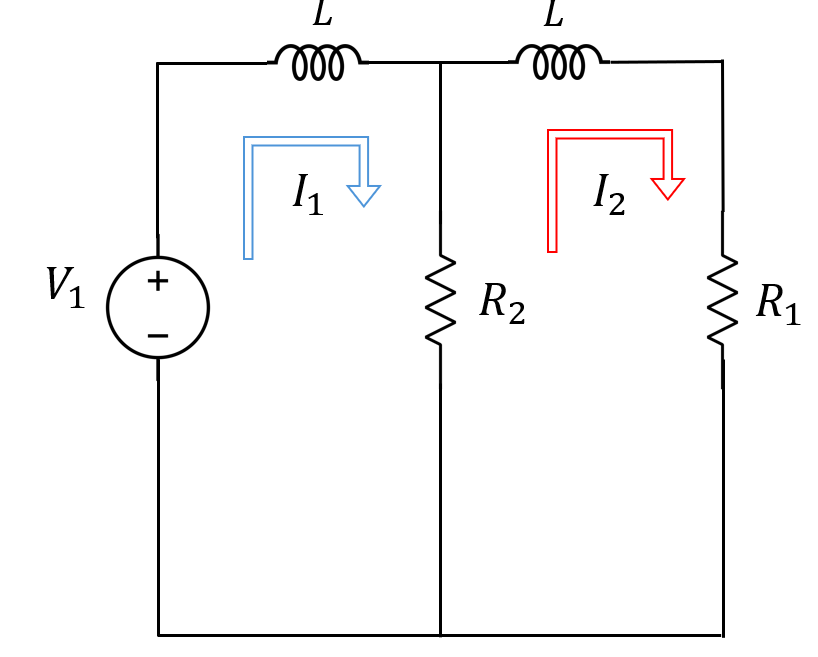
\includegraphics[width=0.6\textwidth]{Examen_1}
    \end{center}
    \begin{center}
        \textbf{Figura 4} Diagrama fasorial para el punto de operación
    \end{center}
    Por lo que el generador se encuentra sobreexcitado
    \end{solution}
    %---------------------------------------------------------------
\end{questions}
\newpage
%%%%%%%%%%%%%%%%%%%%%%%%%%%


\end{document}